\documentclass[conference]{IEEEtran}
\IEEEoverridecommandlockouts
\usepackage{cite}
\usepackage{amsmath,amssymb,amsfonts}
\usepackage{graphicx}
\usepackage{textcomp}
\usepackage{xcolor}
\usepackage[utf8]{inputenc}
\usepackage[T1]{fontenc}

\def\BibTeX{{\rm B\kern-.05em{\sc i}\kern-.025em b\kern-.08em
    T\kern-.1667em\lower.7ex\hbox{E}\kern-.125emX}}

\begin{document}

\title{Descarte Inteligente: Identificação de Resíduos e Orientação de Descarte\\ por Visão Computacional, PLN e Agentes}

\author{
\IEEEauthorblockN{\textit{Preencher: nomes dos integrantes}}
\IEEEauthorblockA{Curso de Inteligência Artificial Aplicada \\
AFYA -- UNIMA Maceió \\
Maceió, Brasil}
}

\maketitle

\begin{abstract}
Grande parte do resíduo reciclável é descartada incorretamente porque as pessoas não sabem
identificar o material, a forma de preparo, a cor da lixeira correspondente ou o ponto de
coleta mais próximo. Este trabalho apresenta um sistema que recebe a foto de um resíduo e
uma pergunta em linguagem natural e responde de forma integrada, combinando visão
computacional, processamento de linguagem natural (PLN) e um agente baseado em regras com
busca. A visão computacional usa uma MobileNetV2 com \textit{transfer learning} sobre o
conjunto TrashNet (6 classes), comparada a um baseline de aprendizado de máquina clássico
(HOG + SVM). O PLN reconhece a intenção da pergunta (7 categorias) e extrai entidades
(material, bairro) por um léxico. O agente resolve o material (texto tem prioridade sobre a
visão), aplica uma base de conhecimento (cores de coleta conforme a Resolução CONAMA
nº 275/2001) e, quando necessário, usa busca A* em um grafo de bairros para indicar o ponto
de coleta mais próximo. A CNN atingiu acurácia de 0,871 e F1-macro de 0,865 no teste,
superando o baseline (0,700 / 0,697). O classificador de intenções atingiu F1-macro de 0,94
no teste, e o A* encontrou o caminho ótimo em 100\% dos casos testados, expandindo em média
3,13 nós contra 4,60 do BFS.
\end{abstract}

\begin{IEEEkeywords}
visão computacional, processamento de linguagem natural, agentes inteligentes, busca A*,
reciclagem, transfer learning
\end{IEEEkeywords}

\section{Introdução}

A separação incorreta de resíduos recicláveis é, em grande parte, um problema de informação:
o morador não sabe identificar o material, não sabe se ele é reciclável, não sabe como
prepará-lo para a coleta, não sabe a cor da lixeira correta e não sabe onde entregá-lo. Isso é
especialmente verdadeiro em cidades como Maceió, onde a cobertura de pontos de coleta
seletiva não é amplamente divulgada.

Este trabalho propõe um assistente que recebe, no mesmo fluxo, a foto de um resíduo e uma
pergunta em linguagem natural (por exemplo, ``isso é reciclável?'' ou ``onde eu levo isso?'')
e devolve uma resposta contextualizada. O sistema integra três módulos de IA: (i) visão
computacional para identificar o material a partir da foto; (ii) PLN para entender a intenção
da pergunta e extrair entidades como material citado e bairro; e (iii) um agente baseado em
regras que combina as duas percepções, consulta uma base de conhecimento e, quando a
pergunta é sobre onde descartar, aciona uma busca A* sobre um grafo de bairros simulado de
Maceió.

A contribuição deste trabalho é a integração desses três módulos em um único fluxo de decisão
explicável (cada resposta expõe as regras que a geraram), com avaliação quantitativa de cada
parte isoladamente e também do sistema combinado, incluindo a comparação da CNN com um
baseline de visão computacional clássica e da busca informada (A*) com alternativas não
informadas (BFS) e não heurísticas (custo uniforme).

\section{Fundamentação Teórica e Trabalhos Relacionados}

\textbf{Classificação de resíduos por imagem.} Thung e Yang~\cite{thung2016trashnet}
introduziram o conjunto TrashNet, com imagens de fundo branco de seis classes de resíduos
(papelão, vidro, metal, papel, plástico e rejeito), e avaliaram classificadores clássicos de
aprendizado de máquina sobre características extraídas das imagens. O presente trabalho usa o
mesmo conjunto, mas compara explicitamente esse tipo de abordagem clássica com uma rede
convolucional pré-treinada.

\textbf{Transfer learning com MobileNetV2.} Sandler et al.~\cite{sandler2018mobilenetv2}
propuseram a MobileNetV2, uma arquitetura convolucional eficiente baseada em blocos
residuais invertidos e \textit{bottlenecks} lineares, adequada para \textit{transfer
learning} com poucas imagens por classe, como é o caso do TrashNet.

\textbf{Descritores clássicos de imagem.} Dalal e Triggs~\cite{dalal2005hog} propuseram o
Histograma de Gradientes Orientados (HOG), um descritor amplamente usado antes da popularização
das redes convolucionais. Este trabalho usa HOG combinado a um histograma de cor (HSV) e um
SVM como baseline de comparação para a CNN.

\textbf{Busca heurística.} Hart, Nilsson e Raphael~\cite{hart1968astar} propuseram o algoritmo
A*, que garante caminho ótimo quando a heurística é admissível (nunca superestima o custo
restante). Neste trabalho, a heurística é a distância em linha reta (haversine) até o
bairro-objetivo mais próximo que aceita o material; como o custo real das vias usa essa mesma
distância multiplicada por um fator viário maior que 1, a heurística nunca supera o custo
real e, portanto, é admissível.

\textbf{Legislação de referência.} A Resolução CONAMA nº 275/2001~\cite{conama275} define o
código de cores para a coleta seletiva no Brasil (azul para papel, vermelho para plástico,
amarelo para metal, verde para vidro, entre outras), usado como base de conhecimento do agente.

\section{Metodologia}

\subsection{Visão por computador}

As imagens do TrashNet (6 classes, cardboard, glass, metal, paper, plastic e trash) são
divididas de forma estratificada em treino/validação/teste (70\%/15\%/15\%, semente 42).
Imagens corrompidas são descartadas no carregamento. O modelo principal é uma MobileNetV2
pré-treinada na ImageNet, treinada em duas fases: (1) extração de características, com os
pesos convolucionais congelados e apenas a camada final treinada; (2) \textit{fine-tuning},
liberando as últimas camadas convolucionais com uma taxa de aprendizado menor. O modelo com
melhor acurácia de validação ao longo das épocas é salvo e, só então, avaliado uma única vez
no conjunto de teste. Como baseline de comparação, um descritor HOG concatenado a um
histograma de cor HSV alimenta um SVM com kernel RBF, cujos hiperparâmetros (custo $C$ e
$\gamma$) são escolhidos por busca em grade com validação cruzada.

\subsection{Processamento de linguagem natural}

A pergunta do usuário passa por normalização (minúsculas, remoção de acentuação e pontuação,
expansão de abreviações comuns como ``vc'' e ``pq''). A intenção é reconhecida por um
classificador treinado sobre uma representação TF-IDF combinando n-gramas de palavras (1 a 2)
e n-gramas de caracteres (2 a 5) -- estes últimos dão robustez a erros de digitação. Três
classificadores são comparados por validação cruzada estratificada de 5 \textit{folds}
(Regressão Logística, Naive Bayes e SVM linear calibrado), e o melhor é re-treinado com todos
os dados de treino e avaliado em um conjunto de teste separado (25\%). As entidades
(material citado e bairro) são extraídas por um léxico em que o termo mais longo e específico
tem prioridade -- por exemplo, ``papel engordurado'' é reconhecido como rejeito e não como
papel reciclável.

\subsection{Agente de decisão e busca}

O agente resolve o material em disputa com prioridade do texto sobre a visão: se a pergunta
cita um material, ele prevalece (e uma divergência com a visão é apenas registrada como
ressalva); caso contrário, usa-se a classe prevista pela CNN, desde que a confiança seja de
pelo menos 60\% -- abaixo disso, o agente pede uma nova foto. Quando a margem entre a 1ª e a
2ª classe mais prováveis é menor que 15\%, a resposta inclui uma ressalva sobre a segunda
possibilidade. Definido o material, uma base de conhecimento estática (reciclabilidade, cor
da lixeira conforme a Resolução CONAMA nº 275/2001 e orientações de preparo) responde às
intenções \textit{identificar}, \textit{reciclavel}, \textit{cor\_lixeira} e
\textit{como\_descartar}. Para a intenção \textit{onde\_descartar}, o agente aciona uma busca
A* sobre um grafo de bairros de Maceió (simulado), cujo custo de aresta é a distância
haversine entre bairros vizinhos multiplicada por um fator viário (1,3) e cuja heurística é a
distância haversine até o bairro-objetivo mais próximo que aceita o material -- heurística
admissível, pois o fator viário é sempre maior que 1. Para comparação, o mesmo grafo também é
resolvido por busca de custo uniforme (A* sem heurística) e por busca em largura (BFS, que
minimiza o número de bairros percorridos, ignorando a distância real). Cada resposta do
agente expõe a lista de regras disparadas (R0 a R16), tornando a decisão explicável.

\subsection{Integração e reprodutibilidade}

A aplicação (Streamlit) recebe a foto e a pergunta no mesmo fluxo e delega ao agente, que
aciona visão, PLN e, quando necessário, a busca. Todos os experimentos usam semente fixa (42)
e os números reportados na Seção IV vêm de arquivos gerados automaticamente pelos scripts do
repositório (nunca digitados manualmente), o que permite reproduzir cada métrica a partir de
um clone limpo do código.

\section{Resultados e Discussão}

\subsection{Visão computacional: CNN x baseline}

A Tabela~\ref{tab:cnn_baseline} compara a CNN MobileNetV2 com o baseline HOG+SVM no conjunto
de teste (nunca usado durante o treino). A CNN supera o baseline em acurácia e F1-macro,
confirmando a vantagem de características aprendidas sobre descritores de imagem fixos para
este problema.

\begin{table}[htbp]
\caption{Visão computacional: CNN x baseline (conjunto de teste)}
\begin{center}
\begin{tabular}{lcc}
\hline
\textbf{Modelo} & \textbf{Acurácia} & \textbf{F1-macro} \\
\hline
MobileNetV2 (CNN) & 0,871 & 0,865 \\
HOG + SVM (baseline) & 0,700 & 0,697 \\
\hline
\end{tabular}
\label{tab:cnn_baseline}
\end{center}
\end{table}

A Figura~\ref{fig:curvas_cnn} mostra a evolução da perda e da acurácia por época nas duas
fases de treino. A Figura~\ref{fig:confusao_cnn} mostra a matriz de confusão da CNN no teste:
os erros mais comuns ocorrem entre classes visualmente próximas (por exemplo, papelão
confundido com papel), o que também aparece nos exemplos qualitativos do repositório.

\begin{figure}[htbp]
\centering
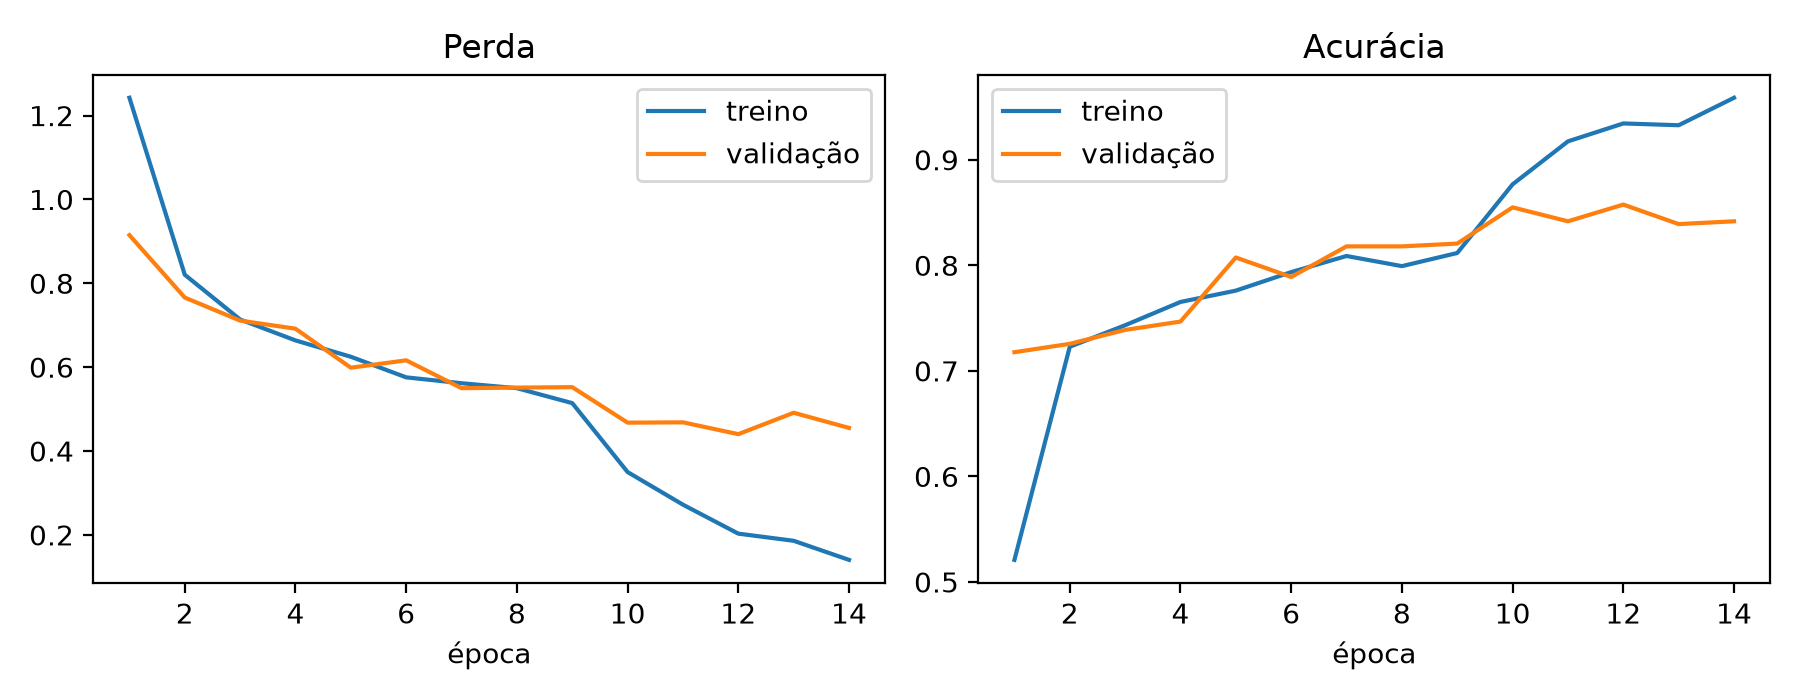
\includegraphics[width=0.95\columnwidth]{../resultados/graficos/curvas_cnn.png}
\caption{Curvas de perda e acurácia da CNN por época (treino e validação).}
\label{fig:curvas_cnn}
\end{figure}

\begin{figure}[htbp]
\centering
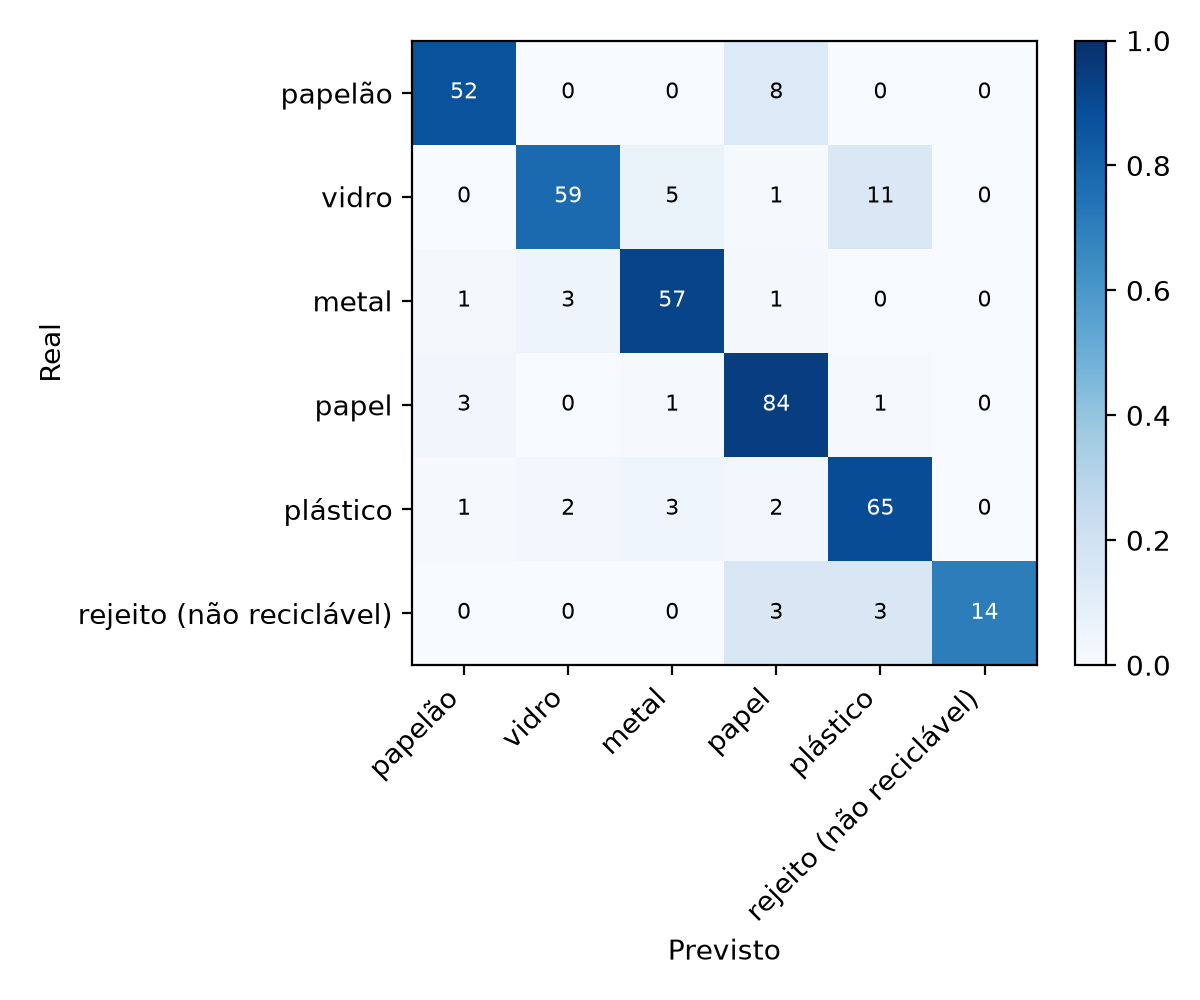
\includegraphics[width=0.95\columnwidth]{../resultados/graficos/confusao_cnn.png}
\caption{Matriz de confusão da CNN no conjunto de teste.}
\label{fig:confusao_cnn}
\end{figure}

\subsection{PLN: comparação de classificadores de intenção}

O conjunto de frases de intenção tem 286 exemplos em 7 categorias, sendo 146 escritos pela
equipe e 140 gerados por IA como complemento (explicitamente marcados por uma coluna de
origem no arquivo de dados), para atingir pelo menos 40 exemplos por categoria. A
Tabela~\ref{tab:intencoes} mostra o F1-macro médio por validação cruzada (5 \textit{folds})
para os três classificadores comparados; a Regressão Logística foi a melhor e, re-treinada
com todos os dados de treino, atingiu acurácia de 0,944 e F1-macro de 0,943 no conjunto de
teste (25\% dos dados, nunca usado no ajuste).

\begin{table}[htbp]
\caption{Comparação de classificadores de intenção (validação cruzada, 5 \textit{folds})}
\begin{center}
\begin{tabular}{lc}
\hline
\textbf{Classificador} & \textbf{F1-macro (média $\pm$ desvio)} \\
\hline
Regressão Logística & 0,888 $\pm$ 0,057 \\
SVM linear (calibrado) & 0,881 $\pm$ 0,065 \\
Naive Bayes (ComplementNB) & 0,874 $\pm$ 0,064 \\
\hline
\end{tabular}
\label{tab:intencoes}
\end{center}
\end{table}

Esse resultado deve ser interpretado com cautela: frases geradas por IA tendem a ser mais
homogêneas entre si do que frases reais escritas por pessoas diferentes, o que facilita a
tarefa do classificador e pode inflar a métrica em relação ao que se observaria com uma
base inteiramente coletada de usuários reais, com gírias e erros de digitação mais
diversos. Ainda assim, o ganho relativo ao conjunto original (F1-macro de teste subindo de
0,696 para 0,943) é coerente com o esperado ao reduzir drasticamente a escassez de dados por
classe (de cerca de 20 para mais de 40 exemplos por intenção).

\begin{figure}[htbp]
\centering
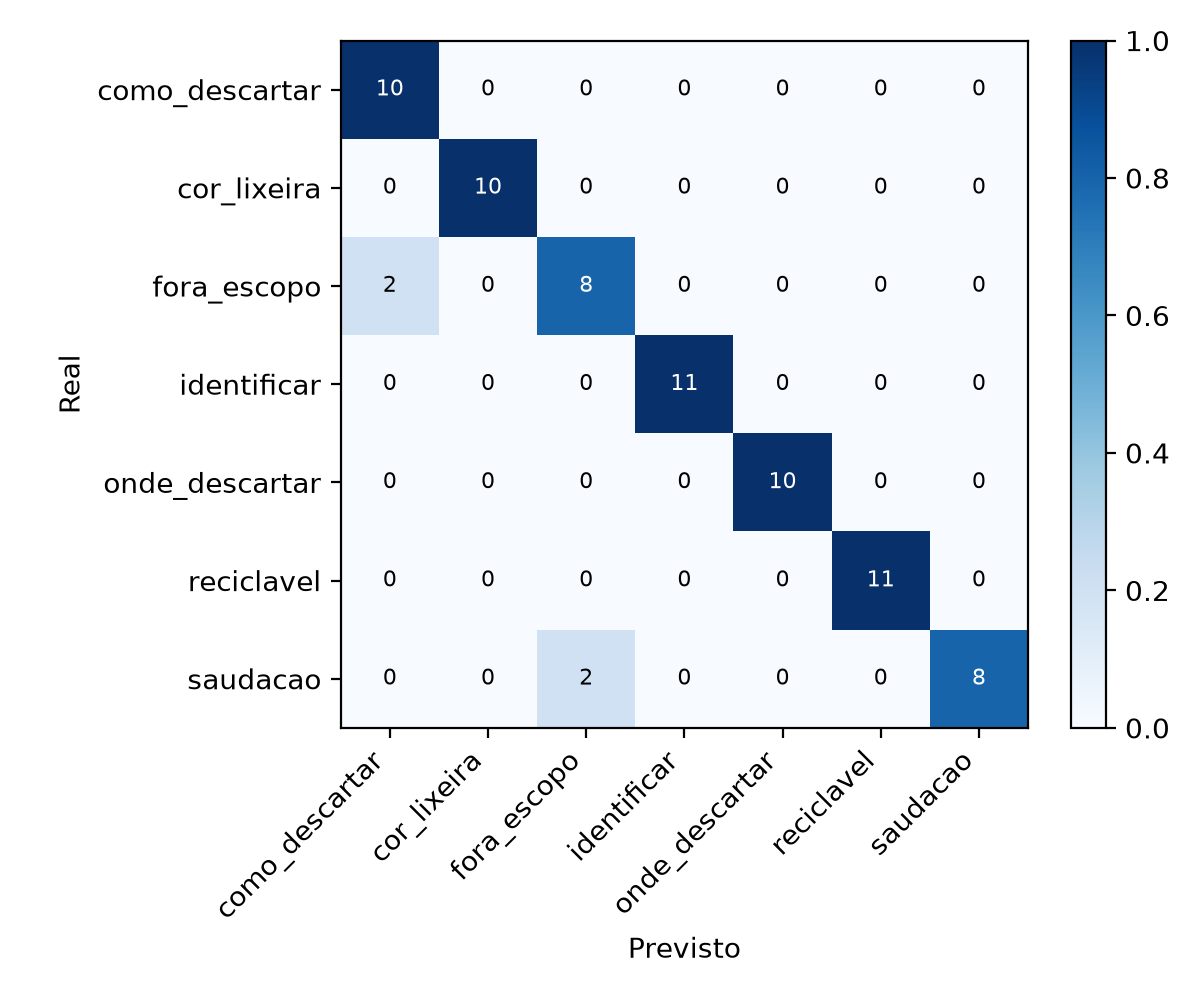
\includegraphics[width=0.95\columnwidth]{../resultados/graficos/confusao_intencoes.png}
\caption{Matriz de confusão do classificador de intenções no conjunto de teste.}
\label{fig:confusao_intencoes}
\end{figure}

\subsection{Busca: A* x custo uniforme x BFS}

A Tabela~\ref{tab:busca} compara as três estratégias de busca em todas as combinações de
bairro de origem e material testadas no grafo de bairros de Maceió. O A* encontra o caminho
ótimo em 100\% dos casos (como garantido pela admissibilidade da heurística), expandindo em
média menos da metade dos nós do BFS, que, por ignorar a distância real, só encontra o
caminho mais curto em 74,5\% dos casos. O custo uniforme também garante otimalidade (é um
caso particular do A* com heurística nula), mas expande mais nós que o A*, evidenciando o
ganho da heurística informada.

\begin{table}[htbp]
\caption{Comparação dos algoritmos de busca no grafo de bairros}
\begin{center}
\begin{tabular}{lccc}
\hline
\textbf{Algoritmo} & \textbf{Nós expandidos} & \textbf{Dist. média (km)} & \textbf{\% ótimo} \\
\hline
A* & 3,13 & 3,29 & 100,0 \\
Custo uniforme & 4,76 & 3,29 & 100,0 \\
BFS & 4,60 & 3,66 & 74,5 \\
\hline
\end{tabular}
\label{tab:busca}
\end{center}
\end{table}

\begin{figure}[htbp]
\centering
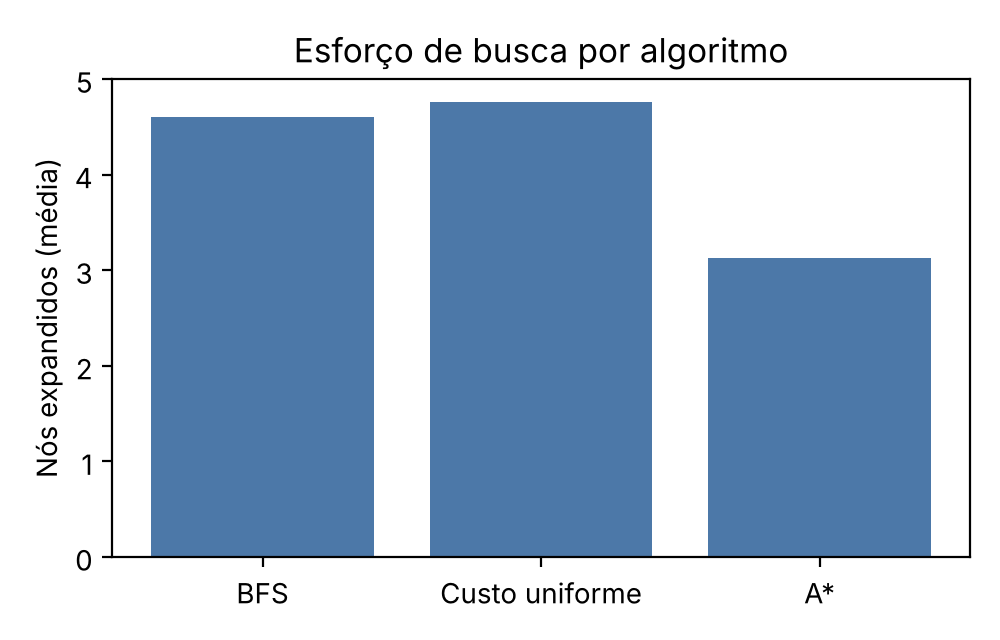
\includegraphics[width=0.95\columnwidth]{../resultados/graficos/busca_nos_expandidos.png}
\caption{Nós expandidos por algoritmo de busca.}
\label{fig:busca}
\end{figure}

\subsection{Integração e exemplos qualitativos}

A Figura~\ref{fig:arquitetura} resume o fluxo integrado. Em testes qualitativos com imagens
reais do conjunto de teste (nunca vistas no treino) e perguntas variadas, o agente respondeu
corretamente às intenções de identificação, reciclabilidade, cor da lixeira, preparo para
descarte e localização do ponto de coleta, expondo em cada caso as regras R0--R16 que
geraram a resposta. Um dos exemplos evidencia uma limitação real da CNN: uma caixa de
papelão foi classificada como papel com 67\% de confiança (margem de 46\% para a segunda
classe), o que ilustra a proximidade visual entre essas duas classes no TrashNet e reforça a
utilidade do limiar de confiança e da ressalva por margem pequena implementados no agente.

\begin{figure}[htbp]
\centering
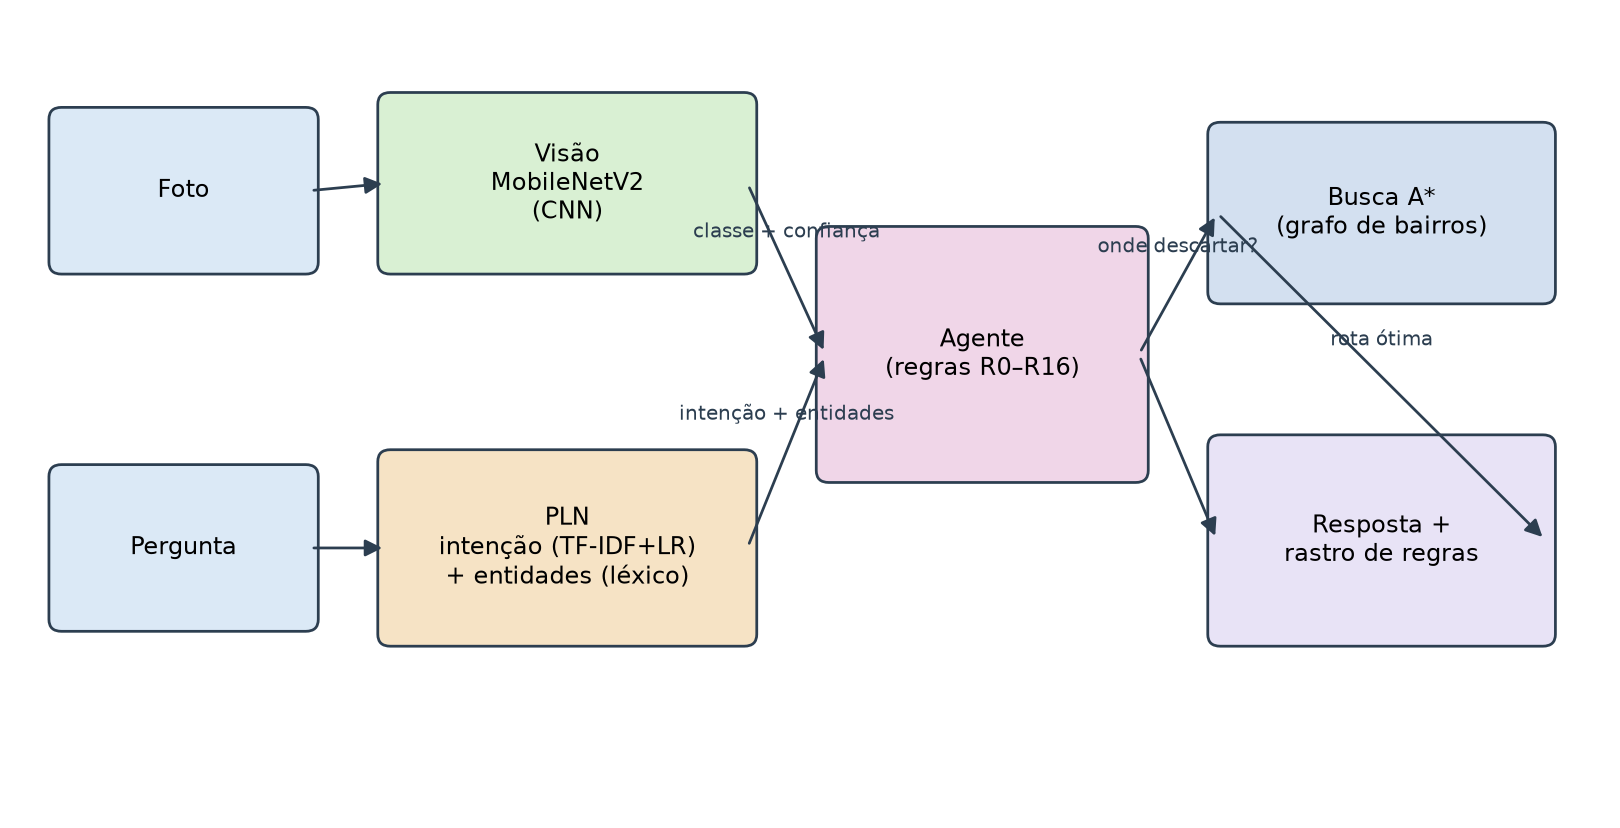
\includegraphics[width=0.95\columnwidth]{../resultados/graficos/arquitetura.png}
\caption{Arquitetura integrada: visão computacional e PLN alimentam o agente de decisão, que consulta a base de conhecimento e, quando necessário, aciona a busca A*.}
\label{fig:arquitetura}
\end{figure}

\section{Conclusão e Trabalhos Futuros}

Este trabalho apresentou um assistente de descarte de resíduos que integra visão
computacional, PLN e um agente baseado em regras com busca informada, avaliando cada módulo
isoladamente com métricas reprodutíveis. A CNN com \textit{transfer learning} superou
claramente o baseline clássico (F1-macro 0,865 x 0,697); o classificador de intenções
atingiu F1-macro de 0,943 no teste, com a ressalva de que parte do ganho vem de dados
gerados por IA, mais homogêneos que frases reais; e a busca A* confirmou, na prática, a
garantia teórica de otimalidade da heurística admissível, expandindo menos nós que as
alternativas.

Como trabalhos futuros, destacam-se: (i) substituir progressivamente as frases geradas por
IA por frases reais coletadas de usuários distintos, com gírias e erros de digitação mais
diversos, para validar se o ganho de F1 se mantém fora de um conjunto mais homogêneo;
(ii) avaliar o modelo de visão em fotos reais de celular, fora do domínio de fundo branco do
TrashNet, e medir a queda de desempenho esperada pela mudança de domínio, bem como a taxa de
recusa do agente (pedidos de nova foto) nesse cenário; (iii) substituir o grafo de bairros e
os pontos de coleta simulados por dados oficiais de Maceió, citando a fonte; e (iv) estender
as classes de resíduos para itens de descarte especial não cobertos pelo TrashNet (pilhas,
eletrônicos, óleo, lâmpadas).

O código-fonte completo, os dados de configuração, os scripts de treino e avaliação e os
resultados usados neste artigo estão disponíveis publicamente em:
\textit{preencher: link do repositório no GitHub}.

\bibliographystyle{IEEEtran}
\bibliography{referencias}

\end{document}
